\bookchapter{บทที่ 49: ติดตั้งสภาพแวดล้อมการพัฒนา — Android Studio กับโปรเจกต์แรกของคุณ}

\chapterintro{ก่อนทำงานให้เป็น ต้องลับเครื่องมือให้คมก่อน บทนี้เราจะสร้าง “ห้องครัว” ให้พร้อม: ติดตั้ง Android Studio รันโปรแกรมจำลองให้ได้ สร้างโปรเจกต์ Android แรกในชีวิต แล้วแกะโครงสร้างโปรเจกต์ดูให้เห็นกับตา พอตั้งสภาพแวดล้อมเสร็จ คุณจะได้เห็นเป็นครั้งแรกว่าโค้ดที่เขียนเองกลายเป็นปุ่มที่กดได้จริง — หลายคนจำวินาทีนั้นได้ตลอดชีวิต}

\booksection{ติดตั้ง Android Studio}

Android Studio คือ IDE แบบครบวงจรอย่างเป็นทางการของ Google ฟรี และรวมทุกอย่างไว้ในตัว: เขียนโค้ด ดูพรีวิวหน้าจอ ดีบัก แพ็กไฟล์ ทำได้ครบในโปรแกรมเดียว ติดตั้ง 4 ขั้นตอน:

\begin{enumerate}
  \item เปิดเว็บทางการ developer.android.com/studio แล้วดาวน์โหลดเวอร์ชันเสถียรล่าสุด (สิงหาคม 2026 คือเวอร์ชันหลังจาก Narwhal มีทั้ง Windows/Mac/Linux);
  \item รันไฟล์ติดตั้งแล้วกด "ถัดไป" ไปเรื่อย ๆ — ตัวติดตั้งจะหยิบ Android SDK กับคอมโพเนนต์โปรแกรมจำลองมาให้เองอัตโนมัติ;
  \item ครั้งแรกที่เปิดโปรแกรม ให้ดาวน์โหลดคอมโพเนนต์ SDK ตามที่ขึ้นบอก (เอาตามค่าเริ่มต้นที่ติ๊กไว้ก็พอ อาจใช้เวลาไม่กี่นาทีและพื้นที่หลาย GB);
  \item พอเสร็จ คุณจะเห็นหน้าต้อนรับ — ยินดีด้วย "ห้องครัว" พร้อมแล้ว
\end{enumerate}

\begin{tcbwarn}{ข้อควรรู้: เช็กสเปกเครื่องให้อยู่ในมือ}
Android Studio เป็นตัว “กินแรม” ตัวยง: แนะนำแรม 16GB ขึ้นไป (8GB ก็รันได้ แต่พอเปิดโปรแกรมจำลองจะกระตุกหน่อย) จองพื้นที่ดิสก์ไว้ 20GB ขึ้นไป และ CPU ต้องรองรับการจำลองเสมือน (เปิด VT-x/AMD-V ใน BIOS) ถ้าคอมเก่าจริง ๆ ใช้ “ดีบักบนเครื่องจริง” แทนโปรแกรมจำลองได้ (จะเล่าในหัวข้อที่ 4 ของบทนี้) ประสบการณ์ใช้งานกลับลื่นกว่า

\end{tcbwarn}

\booksection{สร้างโปรเจกต์แรกของคุณ}

ที่หน้าต้อนรับกด New Project เลือกเทมเพลต Empty Activity (เทมเพลตที่สะอาดที่สุดสำหรับมือใหม่) แล้วกรอกสามอย่างนี้:

\begin{center}
\begin{tabularx}{\linewidth}{|X|X|X|}
\hline
\textbf{รายการตั้งค่า} & \textbf{กรอกอะไร} & \textbf{คำอธิบาย} \tabularnewline
\hline
Name & My First App & ชื่อแอป แสดงบนหน้าโฮมของมือถือ \tabularnewline
Package name & com.example.myfirstapp & ตัวระบุที่ไม่ซ้ำทั่วโลก ธรรมเนียมคือ "เขียนโดเมนกลับด้าน" ตอนนี้ใช้ค่าเริ่มต้นไปก่อน \tabularnewline
Minimum SDK & API 26(Android 8.0) & เวอร์ชันขั้นต่ำที่รองรับ ครอบคลุมอุปกรณ์ 95\%+ \tabularnewline
\hline
\end{tabularx}
\end{center}

\begin{center}\small\color{gray}สามอย่างที่ต้องกรอกตอนสร้างโปรเจกต์\end{center}

พอกด Finish Android Studio จะใช้ Gradle ดาวน์โหลดไลบรารีที่ต้องใช้และบิลด์โปรเจกต์ให้อัตโนมัติ (ครั้งแรกต้องรอสักไม่กี่นาที ครั้งต่อ ๆ ไปจะเร็วขึ้นเยอะ) บิลด์เสร็จ คุณก็มีแอปที่รันได้แล้ว — แม้ตอนนี้มันยังแสดงแค่บรรทัดเดียวว่า “Hello Android!”

\begin{tcbinfo}{เคล็ดลับ: เรื่องที่ต้องรู้เรื่องชื่อแพ็กเกจ}
ชื่อแพ็กเกจ (package name) เหมือน “เลขบัตรประชาชน” ของแอป ห้ามซ้ำกันทั่วโลก และเปลี่ยนไม่ได้อีกแล้วหลังขึ้นสโตร์ ใช้ com.example.xxx ไว้ฝึกหัดส่วนตัวก็พอ แต่ของจริงต้องเปลี่ยนเป็นโดเมนของคุณเองเขียนกลับด้าน (เช่น com.ชื่อคุณ.ชื่อแอป) อย่าเอา com.example ขึ้นสโตร์เด็ดขาด — ร้านค้าจะไม่รับ

\end{tcbinfo}

\booksection{ทำให้รันได้: โปรแกรมจำลองกับเครื่องจริง}

โค้ดเขียนเสร็จ ก็ต้องหา “มือถือ” มารัน คุณมีสองทางเลือก:

\booksubsection{1) โปรแกรมจำลอง (Emulator)}

โปรแกรมจำลองคือการจำลองมือถือ Android ขึ้นมาในเครื่องคอม ใน Android Studio เปิด Device Manager Create Device เลือกเครื่องสักเครื่อง (แนะนำสาย Pixel) เลือกไฟล์ภาพระบบ (แบบที่มาพร้อม Google APIs) ดาวน์โหลด เปิดเครื่อง จากนั้นกดสามเหลี่ยมเขียว Run บนแถบเครื่องมือ อีกไม่กี่วินาที แอปของคุณก็โผล่บนหน้าจอ “มือถือ”

\booksubsection{2) ดีบักบนเครื่องจริง (แนะนำมากกว่า)}

เครื่องจริงคือสภาพแวดล้อมทดสอบที่จริงที่สุดเสมอ — ลูกแรกตอนปัดหน้าจอ เน็ตจริง เซ็นเซอร์จริง โปรแกรมจำลองเทียบไม่ติด การดีบักบนมือถือ Android จริงทำได้ง่าย ๆ:

\begin{enumerate}
  \item บนมือถือเปิด [การตั้งค่า] [เกี่ยวกับโทรศัพท์] แตะ "หมายเลขเวอร์ชัน" ติดกัน 7 ครั้ง เพื่อเปิด "ตัวเลือกนักพัฒนา";
  \item ใน [ตัวเลือกนักพัฒนา] เปิด USB debugging;
  \item เสียบสายข้อมูลเชื่อมเข้าคอม พอมือถือเด้งหน้าต่างถาม ให้เลือก "อนุญาต USB debugging";
  \item กลับไปที่ Android Studio มือถือของคุณจะโผล่ในรายการอุปกรณ์บนแถบเครื่องมือ กด Run ได้เลย
\end{enumerate}

\textbf{ข้อควรระวัง: อย่าเปิด USB debugging ค้างไว้ตลอด}\par

การเปิด USB debugging เหมือนเปิด “ประตูหลัง” ให้คอมพิวเตอร์ ตอนชาร์จในที่สาธารณะหรือเสียบกับคอมที่ไม่น่าเชื่อถือ ต้องปิด USB debugging เสมอ กันคนอื่นอ่านข้อมูลของคุณผ่านมัน ใช้เสร็จตอนพัฒนาก็ปิดทันที ทำให้เป็นนิสัย

\booksection{แกะโครงสร้างโปรเจกต์: แต่ละไฟล์ทำหน้าที่อะไร}

ครั้งแรกที่เปิดโปรเจกต์ แผนผังไฟล์ฝั่งซ้ายอาจทำให้คุณตาลาย ไม่ต้องตกใจ งานพัฒนาประจำวัน 90\% ของคุณ มีคู่หูแค่ตัวที่อยู่ด้านล่างนี้:

\begin{center}
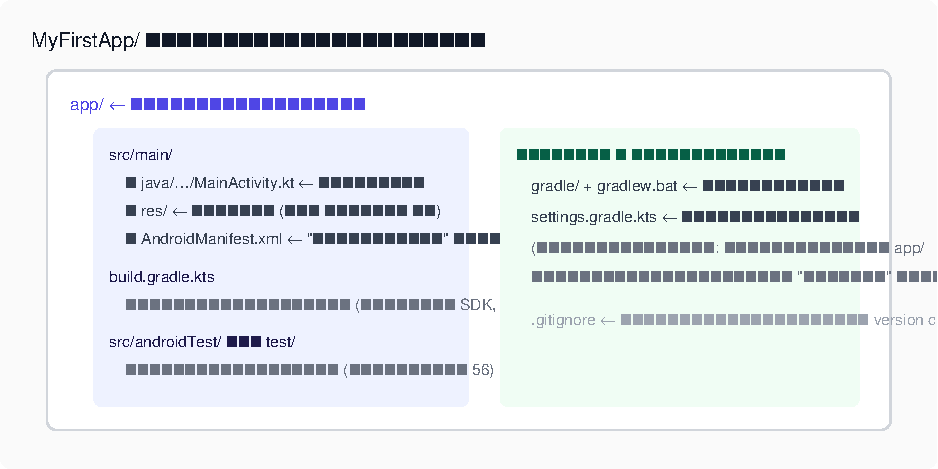
\includegraphics[width=0.92\linewidth]{figures/fig-di-si-shi-jiu-zhang-1}
\\[2pt]\small ภาพที่ 2: โครงสร้างโปรเจกต์ที่มือใหม่ต้องรู้ (จำง่าย ๆ: แตะแค่โฟลเดอร์ app/)
\end{center}

\begin{itemize}
  \item MainActivity.kt: "ประตูหลัก" ของแอป ผู้ใช้กดไอคอนเปิด ตัวแรกที่ถูกปลุกคือมัน ในเทมเพลตปัจจุบันมันทำหน้าที่แสดง "Hello Android!"
  \item AndroidManifest.xml: "ทะเบียนบ้าน" ของแอป — ประกาศว่าแอปนี้ชื่ออะไร ใช้ไอคอนตัวไหน มีหน้าอะไรบ้าง และต้องขอสิทธิ์อะไร (กล้อง ระบุตำแหน่ง ฯลฯ)
  \item โฟลเดอร์ res/: คลังทรัพยากร เก็บรูปภาพ ไอคอน ข้อความ สี เก็บข้อความไว้ในไฟล์ทรัพยากรแทนที่จะเขียนฝังไว้ในโค้ด เป็นนิสัยที่ดีของการพัฒนา Android (เปลี่ยนภาษา เปลี่ยนธีมก็ง่าย)
  \item build.gradle.kts: สูตรการบิลด์ — ประกาศเวอร์ชันขั้นต่ำที่รองรับ และใช้ไลบรารีอะไรบ้าง (เช่น Compose)
\end{itemize}

\booksection{ลองมือกันหน่อย: เปลี่ยน “Hello” เป็นชื่อของคุณ}

เปิด MainActivity.kt คุณจะเห็นโค้ดที่เทมเพลต Compose สร้างไว้ หาบรรทัด Text(“Hello Android!”) แล้วเปลี่ยนข้อความในเครื่องหมายคำพูดเป็นชื่อของคุณ เช่น Text(“สวัสดี สมชาย! นี่คือแอปแรกของฉัน”) จากนั้นกด Ctrl+R (บน Mac คือ Cmd+R) รันใหม่ อีกไม่กี่วินาที โปรแกรมจำลองก็แสดงชื่อของคุณให้เห็น

\begin{lstlisting}[language=Kotlin]
setContent {
    MyFirstAppTheme {
        Surface(modifier = Modifier.fillMaxSize()) {
            // v แก้ตรงนี้เป็นข้อความของคุณเอง
            Text("สวัสดี ซานผวน! นี่คือแอปแรกของฉัน")
        }
    }
}
\end{lstlisting}

ยินดีด้วย คุณเพิ่งวนจบหนึ่งรอบ “แก้โค้ด คอมไพล์ ติดตั้ง รัน” แบบสมบูรณ์ วงจรนี้แหละคือชีวิตประจำวันของการพัฒนาในทุกวันข้างหน้า รีบต่อความมันส์ต่อเลย ลองแก้อย่างอื่นดูอีก: ขยายตัวอักษรให้ใหญ่ขึ้น เปลี่ยนสี — บทต่อไปเราจะเรียนว่า “เวทมนตร์” เหล่านี้มาจากไหน

\booksection{หน้าด่านเจอ error ที่พบบ่อย: “ห้องฉุกเฉิน” ของมือใหม่สองสัปดาห์แรก}

ช่วงตั้งสภาพแวดล้อมและบิลด์ครั้งแรก คุณมีโอกาสสูงมากที่จะเจอ error สามแบบนี้ ไม่ต้องตกใจ มียาแก้ทุกตัว:

\begin{center}
\begin{tabularx}{\linewidth}{|X|X|X|}
\hline
\textbf{อาการ error} & \textbf{สาเหตุที่พบบ่อย} & \textbf{ยาแก้} \tabularnewline
\hline
Gradle sync failed / ดาวน์โหลดไลบรารีช้า & เครือข่ายเข้าถึง repository ไม่คล่อง & ตั้งค่า Gradle ให้ใช้ repository มิเรอร์ที่เร็วในภูมิภาค (มิเรอร์ maven อย่าง Aliyun/Tencent Cloud) ค้นเว็บหา "gradle mirror" แล้วทำตาม \tabularnewline
คอมโพเนนต์ SDK ขาดหาย & ตอนติดตั้งข้ามการดาวน์โหลด SDK & ไปที่ Settings SDK Manager ติดตั้งเพลตฟอร์มกับเครื่องมือที่ขาดให้เรียบร้อย \tabularnewline
โปรแกรมจำลองเปิดไม่ขึ้น / จอดำ & ยังไม่ได้เปิดการจำลองเสมือน หรือไฟล์ภาพระบบเสียหาย & เปิด VT-x/AMD-V ใน BIOS; ลบโปรแกรมจำลองทิ้งแล้วสร้างใหม่; หรือใช้ดีบักบนเครื่องจริงไปเลย \tabularnewline
\hline
\end{tabularx}
\end{center}

\begin{center}\small\color{gray}ตารางหน้าด่าน error ตอนตั้งสภาพแวดล้อมสำหรับมือใหม่\end{center}

\begin{tcbinfo}{เคล็ดลับ: วิธีค้นหา error}
บรรทัดแรกของข้อความ error มีค่าที่สุด — คัดลอกตามตัวไปใส่ในเสิร์ชเอนจิน แล้วเติมคำว่า “android studio” อย่าค้นคำกว้าง ๆ ว่า “ติดตั้งสภาพแวดล้อมไม่ได้ทำยังไงดี” ให้ค้นคำเจาะจงอย่าง “Gradle sync failed: Could not resolve com.android.tools.build” คำถามแม่นยำเท่านั้น จึงจะได้คำตอบแม่นยำ

\end{tcbinfo}

\begin{tcbpractice}{ลงมือทำด้วยกัน: ทำเช็กลิสต์ "พิธีกรรมนักพัฒนา" ของคุณให้ครบ}
1) ติดตั้ง Android Studio และรันโปรแกรมจำลองให้ได้; 2) รันแอปของตัวเองบนเครื่องจริงสักครั้งและแคปหน้าจอเก็บไว้; 3) เปลี่ยนข้อความ Hello เป็นชื่อของคุณ; 4) บีบอัดโปรเจกต์เก็บสำรองไว้ ทำครบสี่ข้อนี้ คุณก็ประกาศได้เต็มปากว่า: ฉันก็เป็นนักพัฒนา Android แล้ว (มีภาพแคปเป็นหลักฐาน)

\end{tcbpractice}

\begin{tcbsummary}{สรุปบทนี้}
\begin{itemize}
  \item Android Studio = IDE ฟรีอย่างเป็นทางการ; แนะนำแรม 16GB + ดิสก์ 20GB + เปิดการจำลองเสมือน
  \item สามองค์ประกอบของโปรเจกต์ใหม่: ชื่อ, ชื่อแพ็กเกจ (ไม่ซ้ำทั่วโลก อย่าขึ้นสโตร์ด้วย com.example), SDK ขั้นต่ำ (เริ่มที่ API 26)
  \item สองวิธีรัน: โปรแกรมจำลอง (มือถือเสมือนในคอม) กับเครื่องจริง (เปิด USB debugging ใช้เสร็จอย่าลืมปิด)
  \item จำง่าย ๆ เรื่องโปรเจกต์: แตะแค่โฟลเดอร์ app/ — MainActivity.kt คือประตูหลัก, Manifest คือทะเบียนบ้าน, res/ คือคลังทรัพยากร
  \item ชีวิตประจำวันนักพัฒนา = แก้โค้ด Run ดูผล วนซ้ำไปเรื่อย ๆ
\end{itemize}

\end{tcbsummary}
